\documentclass[10pt,a4paper,titlepage]{article}
\usepackage[margin=1.6cm]{geometry}    % margens menores
\usepackage[utf8]{inputenc} % para poder colocar acentos e caracteres especiais
\usepackage[portuguese]{babel}
\usepackage{graphicx} % Permite inserir e manipular imagens
\usepackage{fancyhdr} % 
\usepackage{caption}
\usepackage{geometry} % Permite definir facilmente margens e o layout da página
\usepackage{setspace} % Permite alterar o espaçamento entre linhas
\usepackage{titlesec} % Permite personalizar os títulos de secções e subseções
\usepackage[hidelinks]{hyperref} % Ativa links clicáveis no PDF
\usepackage{multicol} % coloca isto no preâmbulo

% Page setup
\geometry{margin=2.5cm}
\setstretch{1.5}
\pagestyle{fancy}
\fancyhf{}
\rhead{\thepage}
\lhead{Escola Superior de Tecnologia e Gestão}

% Title formatting
\titleformat{\section}{\large\bfseries}{\thesection}{1em}{}
\titleformat{\subsection}{\normalsize\bfseries}{\thesubsection}{1em}{}

\begin{document}
	
\thispagestyle{empty} % ignorar cabeçalho na primeira página


% --- Bloco de Título Compacto ---
\begin{center}
	{\Large \textbf{Trabalho Prático CDN}} \\ \vspace{0.2cm}
	\small Diogo Pereira (8200594) $\cdot$ Duarte Sampaio (8190553) $\cdot$ Hugo Guimarães (8220337) \\ \vspace{0.2cm}
	\small 14/12/2025
\end{center}
\hrule % Linha horizontal para separar do texto
\vspace{0.5cm} % Espaço antes de começar o texto
% --------------------------------


\section{Justificação da Arquitetura Adotada}

Na Figura \ref{fig:diagrama_arquitetura} está representada a arquitetura da aplicação desenvolvida no AWS, e como é possível visualizar, ela encontra-se devidida nas duas principais camadas: o frontend e o backend.

\begin{figure}[h]
	\centering
	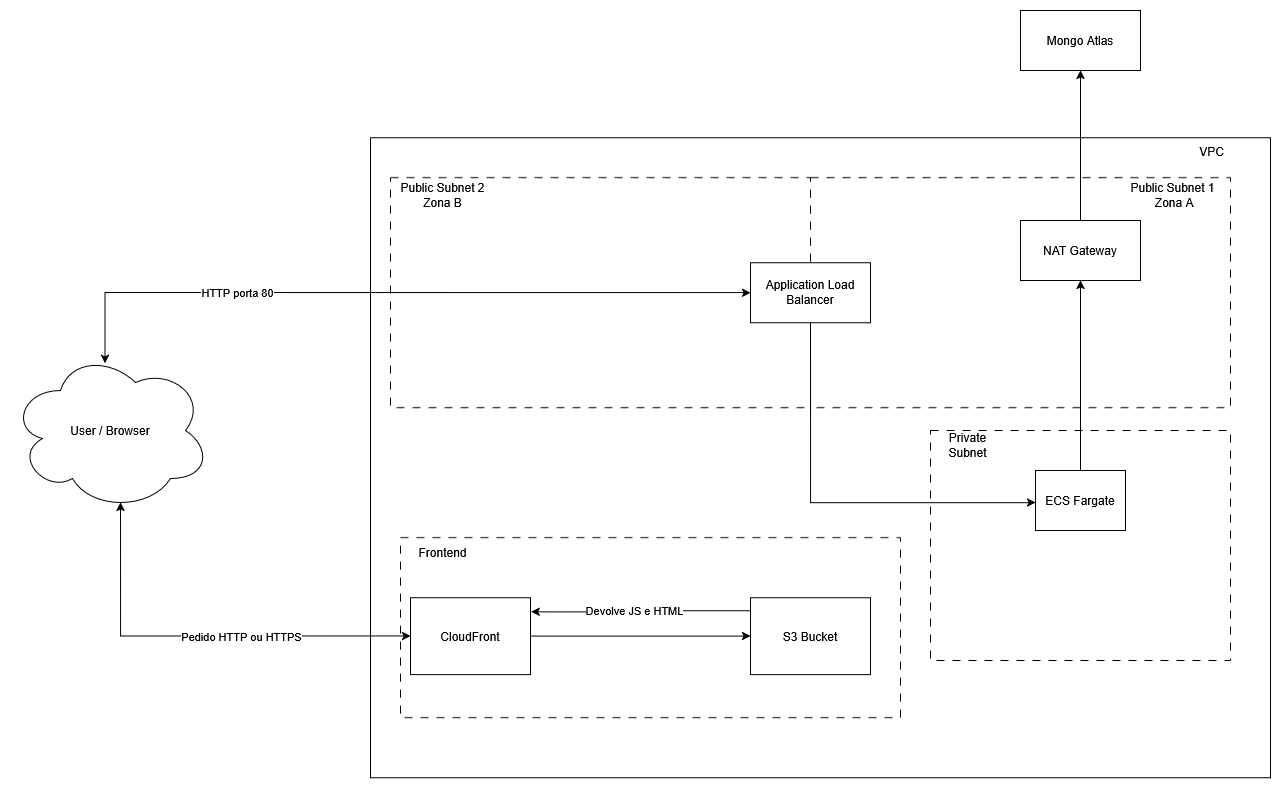
\includegraphics[width=0.8\linewidth]{imagens/Diagrama_CDN}
	\caption{Diagrama de Arquitetura}
	\label{fig:diagrama_arquitetura}
\end{figure}

\begin{itemize} 
	\item \textbf{Frontend:} Este está num \textit{bucket} S3 privado e acessível via Amazon CloudFront (CDN).
	
	\item \textbf{Backend:} Este está implementado numa VPC (\textit{Virtual Private Cloud}) segmentada. A API executa sobre Amazon ECS com Fargate, estando numa subnet privada de modo a estar totalmente isolada da internet. O tráfego de entrada é gerido por um \textit{Application Load Balancer} (ALB) localizado nas duas subnets públicas, e está responsável por encaminhar os pedidos para os containers.
\end{itemize}

O backend comunica com uma base de dados MongoDB, mas esta não existe dentro do AWS, mas sim como um serviço externo, o MongoDB Atlas, portanto o URI de conexão ao mesmo é passado como uma variável de ambiente na configuração do Open Tofu. Estando depois disponível à API através do intermédio da NAT Gateway, que é necessário visto que a API encontra-se numa subnet privada.

\section{Decisão Decisões Tomadas}

\subsection{Porque se usou o EC2 Fargate}
Utilizou-se ECS Fargate porque este é mais simples do que configurar manualmente os servidores em EC2, para além deste ser serverless, debitando somente o que gasta, adequando-se melhor às necessidades do grupo que estão limitados aos créditos que a Amazon oferece.

\subsection{Integração Dinâmica Frontend-Backend}
De modo a facilitar o processo de deploy, fez-se um ficheiro \textit{config.js} no forntend que tem credenciais de acesso à API, mas como o endereço do mesmo só é conhecido após o deploy, então utilizou-se o \textit{aws\_s3\_object} que injeta dinamicamente um ficheiro \textit{config.js} no bucket S3 contendo o endpoint do ALB.

\subsection{Porque se utilizou o MongoDB Atlas}
No começo tentou-se seguir a sugestão do professor de usar o DynamoDB, mas como havia pouco tempo para a realização do trabalho, e não se estava a ter sucesso na implementação do mesmo na API, então decidiu-se utilizar o MongoDB visto que já foi utilizado diversas vezes em outras unidades curriculares.
No entanto, devido à falta de tempo, e ao receio de acabarem os créditos do AWS, decidiu-se utilizar o MongoDB Atlas, e caso houvesse tempo, o que não aconteceu, implementar-se-ia a base de dados diretamente no AWS.
\section{Como Executar a Aplicação}
Como o relatório só pode ter até 3 páginas, então foi colocado na raiz do projeto um ficheiro markdown denominado HOW\_TO\_RUN.md.
\section{Utilização de Inteligência Artificial}
Para o desenvolvimento deste projeto foram utilizadas algumas inteligências artificiais como auxílio ao desenvolvimento do mesmo. No entanto a utilização das mesmas não foi utilizada como substituto do trabalho necessário para a aquisição das competências necessárias para o desenvolver, sendo somente utilizadas como recurso para facilitar trabalho repetitivo, demorado e não relevante para o principal objetivo do projeto. Tendo sido utilizadas para as seguintes tarefas:

\begin{itemize}
	\item Atribuição das classes bootstrap no frontend para ficar mais esteticamente agradável.
\end{itemize}
\section{Referências para a construção do trabalho}

\begin{itemize}
	\item \textbf{Criar um bucket S3 em OpenTofu: } https://medium.com/@2017tejasgupta/created-your-first-s3-bucket-with-opentofu-7c806bbed218

	\item \textbf{Criar um bucket S3 em Terraform e expor com o CloudFront:} https://medium.com/@ssare/make-s3-bucket-public-with-object-read-only-via-terraform-0b71393b963e
	
	\item \textbf{Tabelas de Roteamento:} https://search.opentofu.org/provider/opentofu/aws/latest/docs/resources/route\_table

	\item \textbf{Configuração de ECS Fargate: }
	
	\begin{itemize}
		\item https://medium.com/@olayinkasamuel44/using-terraform-and-fargate-to-create-amazons-ecs-e3308c1b9166
		
		\item https://spacelift.io/blog/terraform-ecs
		https://www.gyden.io/en/content-hub/how-to-setup-amazon-ecs-fargate-using-terraform
		
		\item https://search.opentofu.org/module/cloudposse/ecs-cluster/aws/latest
		
		\item https://search.opentofu.org/provider/opentofu/aws/latest/docs/resources/ecs\_service
		
		\item https://spacelift.io/blog/terraform-ecs
	\end{itemize}
	
	\item \textbf{Configuração de VPC e Subnets:}
	
	\begin{itemize}
		\item https://search.opentofu.org/provider/opentofu/aws/latest/docs/resources/vpc
		\item https://dev.to/vinod827/creating-custom-vpc-on-aws-using-opentofu-3760
		\item https://search.opentofu.org/provider/opentofu/aws/latest/docs/resources/subnet
		\item https://dev.to/vinod827/creating-custom-vpc-on-aws-using-opentofu-3760
	\end{itemize}
	
\end{itemize}



\end{document}